\section{Wearables}\label{sec:wearables} %Working title
%Thalley: Første source kan også laves som en fin graf hvis ønsket. Brug tal fra: http://www.statista.com/statistics/259372/wearable-device-market-value/
Wearable technology is a trending form of technology as of 2015 \cite{WEARABLESTREND}. 
As the name implies, wearables are devices that, unlike most electronics, are worn by the user. 
The most common types of wearables today are smartwatches, 
\ie watches that run an advanced operating system and can perform more actions that regular watches such as communicating with a smartphone or other smart devices, 
and smart wristbands which usually tracks activity, 
among other things, and sends this data to a connected smartphone via an application. 
Smartphones are usually not considered a wearable since they are usually \emph{carried} and not \emph{worn}. 

%Hvorfor wearables?
The increasing trend in wearables is likely due to increased computational power in small devices and decreased sizes of sensors, 
which allows more power and functionality to wearables devices. 
The increasing trend, as well as better wearables devices, 
opens up new possibilities since we can now carry more computational power with us on the go that we can utilize to perform actions that we could not before, 
or perform other actions faster or better. 
Examples of this could be that we can now track our level of activity together with our location to analyze ourselves or even automate actions based on our location, mood or even health. 

%HVad kan en wearable? Hvilke sensorer findes der? Hvad er state of the art? 
If we take a look at some of the current state of the art or the most popular wearable devices right now, 
we can create an image of what we can actually monitor, track, control or in other ways do with devices that we can wear. 
One of the latest and most advanced wearable is the HIRIS \cite{hirisweb}. 
The HIRIS is a wearable computer able to track 3D movements in real-time. 
By using several HIRIS, you can get a create a full-body tracking system. 
Aside from 3D tracking, HIRIS also tracks heart rate and temperature and can connect to other devices and control these. 
Another advanced wearable tracker is the Jawbone UP3 \cite{JAWBONE}. 
This wearable is also able to track your heart rate, activity, sleep and temperature, but unlike the Hiris cannot control any other devices. 
Since one of the most popular wearables is the smartwatch, it makes sense to mention these as well. 
One of most interesting smartwatches, due to developer options, is the Pebble Smartwatch \cite{PEBBLE}. 
This smartwatch works with iPhones and Android smartphones and comes with a variety of applications for tracking fitness and control music among other things. 
Aside from this, the watch also comes with an accelerometer and a magnetometer, meaning that is can track your motions and directions. 

By analyzing the list of 348 different wearables from Vandrico\cite{LISTOFWEARABLES} of September 2015, 
we can see which sensors and components are most common among wearables and where on the body they are worn. 
It is important to note that all of this information comes Vandrico's database, and may differ from other findings. 
\Cref{fig:wearables-category} shows which categories these wearables fit in. The most common one, lifestyle, 
describes wearables such as smartwatches or other devices that are meant to be used and worn on a daily basis. 
Some devices may fit more than one category.

\begin{figure}[!htb]
    \centering
    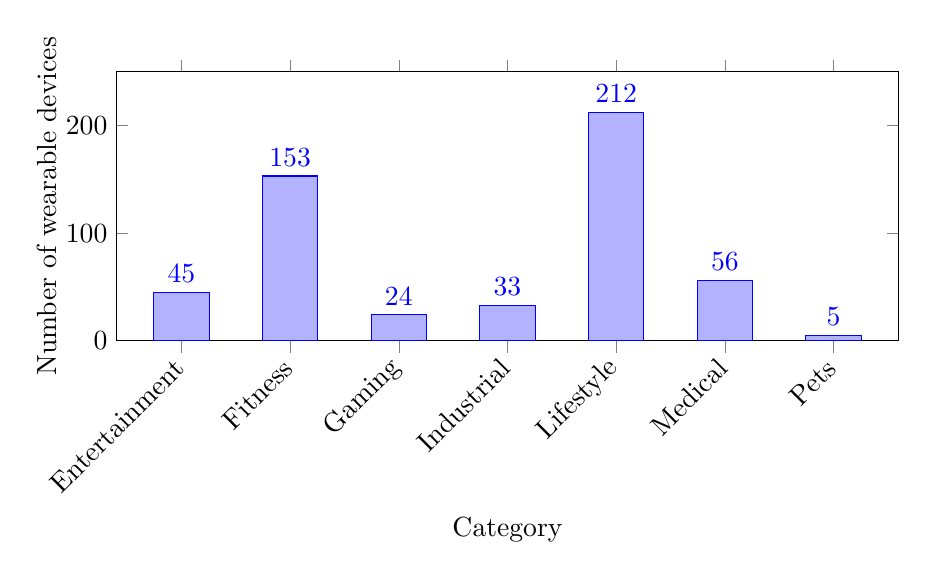
\begin{tikzpicture}
    \begin{axis}[
        height=5cm,
        width=0.95\textwidth,
        xlabel={Category},
        xticklabel style={rotate=45, anchor=east, yshift=-0.5ex},
        ylabel={Number of wearable devices},
        yticklabel style={align=right,inner sep=0pt,xshift=-0.3em},
        nodes near coords align={vertical},
        nodes near coords,
        xtick=data,
        symbolic x coords={Entertainment,Fitness,Gaming,Industrial,Lifestyle,Medical,Pets},
        ybar,
        ymax=250,
        ymin=0,
        bar width=20pt,
        ]
        \addplot coordinates {(Entertainment,45) (Fitness,153) (Gaming,24) (Industrial,33) (Lifestyle,212) (Medical,56) (Pets,5)};
    \end{axis}
\end{tikzpicture}
    \caption{Number of devices in each category}
    \label{fig:wearables-category}
\end{figure}

\Cref{fig:wearables-placement} shows where on the body the wearable should or can be worn. 
The most common placement is the wrist where smartwatches or wristband are worn, 
which are the most popular wearables. The devices that are worn on the head are usually augmented/virtual reality headsets, 
but also includes smart bike-helmets or ear/headphones.

\begin{figure}[!htb]
  \centering
  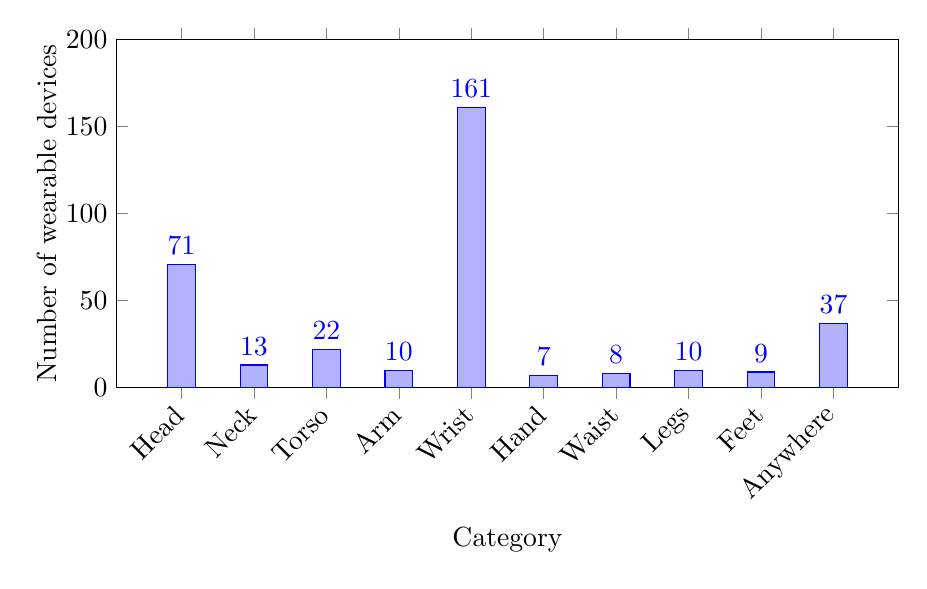
\begin{tikzpicture}
\begin{axis}[
    height=6cm,
    width=0.95\textwidth,
    xlabel={Category},
    xticklabel style={rotate=45, anchor=east, yshift=-0.5ex},
    ylabel={Number of wearable devices},
    yticklabel style={align=right,inner sep=0pt,xshift=-0.3em},
    nodes near coords align={vertical},
    nodes near coords,
    xtick=data,
    symbolic x coords={Head,Neck,Torso,Arm,Wrist,Hand,Waist,Legs,Feet,Anywhere},
    ybar,
    ymax=200,
    ymin=0,
    ]
    \addplot coordinates {(Head,71) (Neck,13) (Torso,22) (Arm,10) (Wrist,161) (Hand,7) (Waist,8) (Legs,10) (Feet,9) (Anywhere,37)};
\end{axis}
  

\end{tikzpicture}
  \caption{Placements of wearables}
  \label{fig:wearables-placement}
\end{figure}

\Cref{fig:wearables-sensors} shows which sensors and components are mostly available in wearables. 
Due to its high usability, the accelerometer is a very important sensor which is found in approximately half the wearables. 
The remaining sensors in \Cref{fig:wearables-sensors} are, unsurprisingly sensors that we also find in smartphones as they give a lot of options when it comes to developing applications. 
\begin{figure}[!htb]
    \centering
    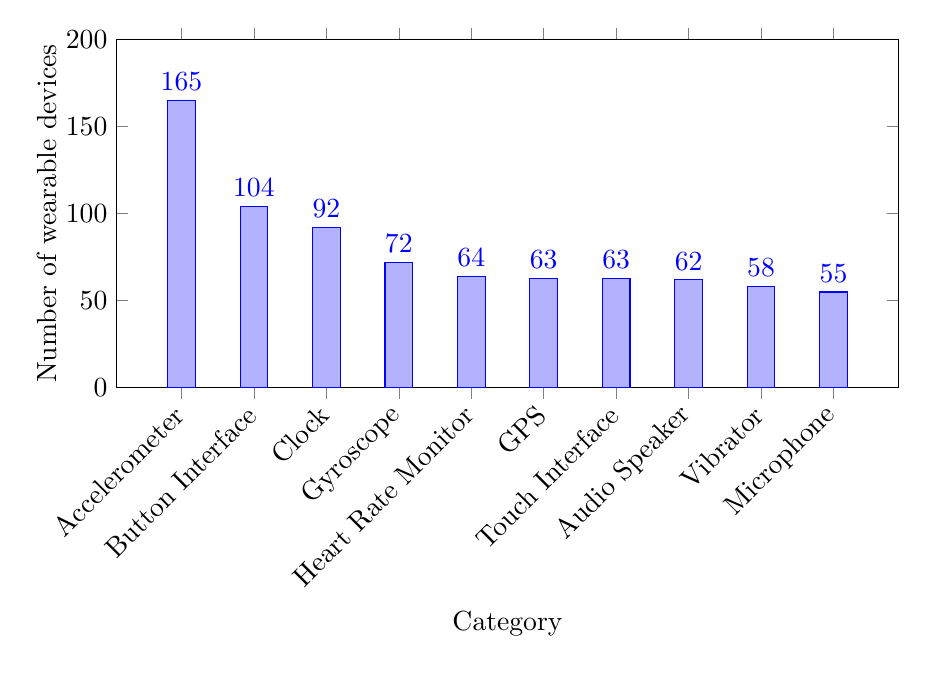
\begin{tikzpicture}
\begin{axis}[
    height=6cm,
    width=0.95\textwidth,
    xlabel={Category},
    xticklabel style={rotate=45, anchor=east, yshift=-0.5ex},
    ylabel={Number of wearable devices},
    yticklabel style={align=right,inner sep=0pt,xshift=-0.3em},
    nodes near coords align={vertical},
    nodes near coords,
    xtick=data,
    symbolic x coords={Accelerometer,Button Interface,Clock,Gyroscope,Heart Rate Monitor,GPS,Touch Interface,Audio Speaker,Vibrator,Microphone},
    ybar,
    ymax=200,
    ymin=0,
    ]
    \addplot coordinates {(Accelerometer,165) (Button Interface,104) (Clock,92) (Gyroscope,72) (Heart Rate Monitor,64) (GPS,63) (Touch Interface,63) (Audio Speaker,62) (Vibrator,58) (Microphone,55)};
\end{axis}
  

\end{tikzpicture}
    \caption{Top 10 mostly used sensors}
    \label{fig:wearables-sensors}
\end{figure}

This section gave a short overview of the current state of wearables, what they are and which sensors are widely available. 
This information should be remembered if developing any system that utilizes wearables. 

%Skab et overblik over de nyeste devices
%Grafer over hvilke sensorere der mest typiske?
%Grafer over kropsdele?
%Hvad er de nyeste teknologier indenfor wearables? 
